%-------------------------------------------------------------
% Main text file
%-------------------------------------------------------------
\documentclass[a4,12pt]{article} % Default font size and left-justified equations 

% style file (.sty) with general report format
\usepackage{General_Header}


\begin{document}


\section*{Spectral Characterisation of Random Rough Surfaces}
Surface roughness is quantitatively described by its height, denoted as $h(\boldsymbol{x})$, with respect to positions $\boldsymbol{x}$. The variation in height is captured by the correlation function $C(\boldsymbol{x}_2 - \boldsymbol{x}_1)$ evaluated between two seperated points. Employing a Fourier transform on this function and invoking the convolution theorem enables surface roughness analysis within the spatial frequency domain, characterised by wave vectors $\boldsymbol{k}$. This approach yields the surface power spectrum $C(\boldsymbol{k})$, also referred to as the power spectral density, which statistically describes the roughness by revealing the amplitude of height variations and the distribution of spatial frequencies $\boldsymbol{k}$ --- the inverse of the wavelength. Surface exhibiting large height variations over short length scales thus will show elevated spatial frequencies in their power spectra compared to smoother surfaces, making the power spectrum a useful tool to characterise surface roughness over diverse length scales.

\begin{figure}
    \centering
    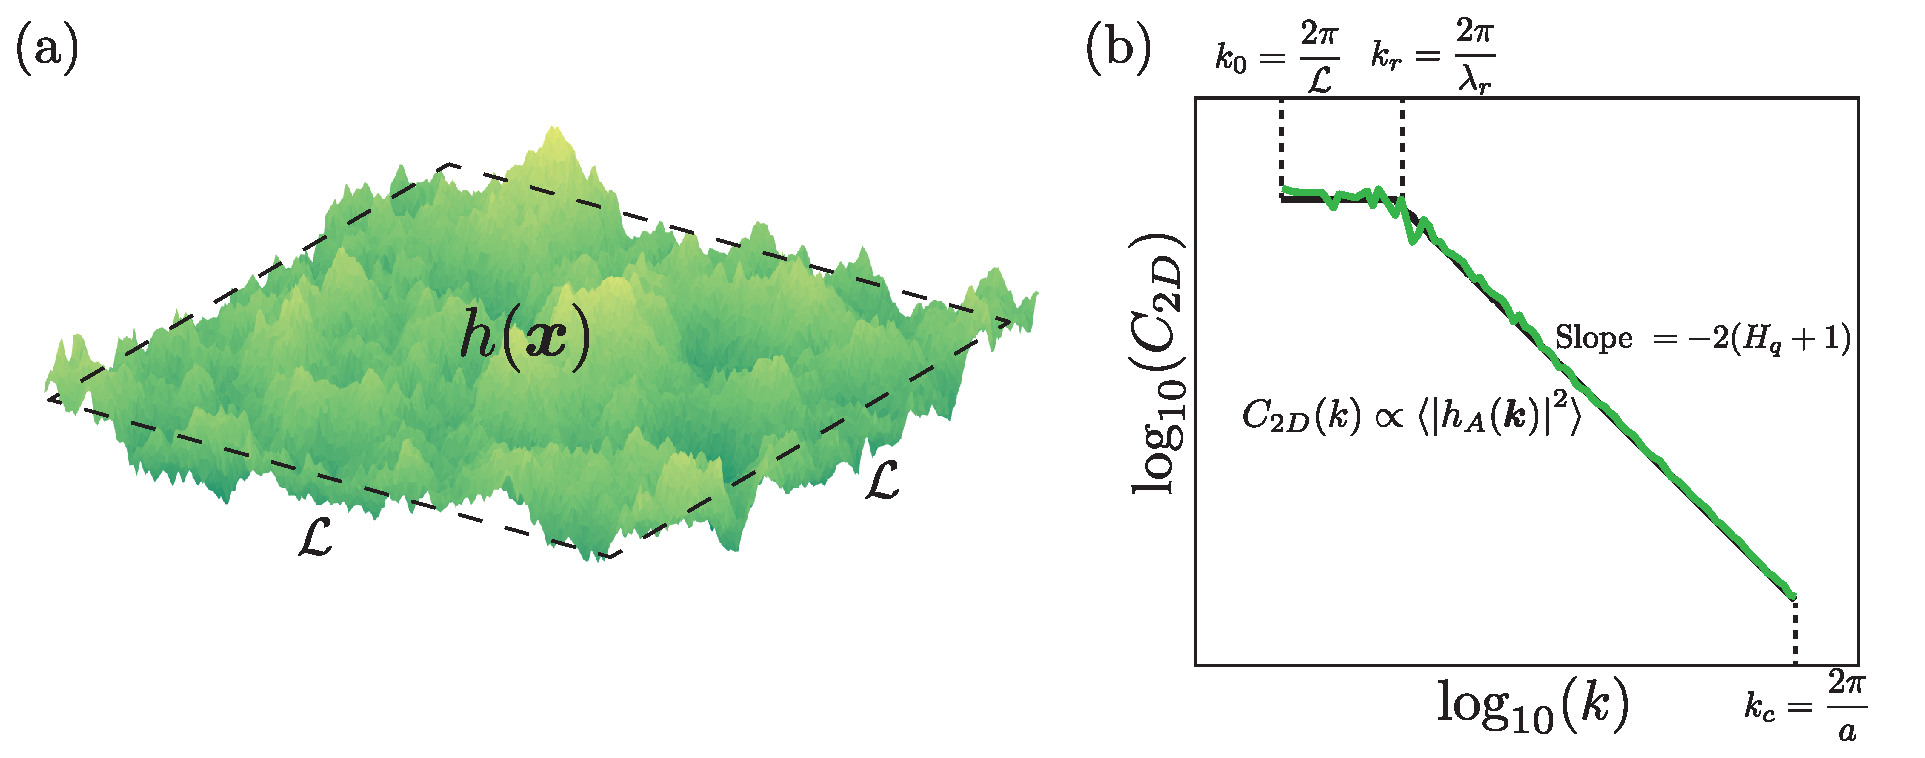
\includegraphics[width=0.95\textwidth]{Figures/fig1.eps}
    \caption{(a) An example of a surface profile $h(\boldsymbol{x})$ with random roughness on a square plane. (b) A typical surface roughness power spectrum associated with the height profile $h(\boldsymbol{x})$, possessing a mean of zero and characterised, on average, by a second moment as defined by the height spectrum. The green line indicates the exact power spectrum taken from the sample in (a). Further details regarding the notations, e.g., Hurst exponent $H_q$, roll-off wavelength $\lambda_r$, and wave vector $k_r$, are common in the literature, such as in Ref.\cite{persson2004nature}.}
    \label{fig:Spectrum}
\end{figure}

If the surface statistical properties are isotropic and translationally invariant, then the dependency of the spectrum on the wave vector reduces to the magnitude, i.e., $C(\boldsymbol{k}) = C(k)$. For simplicity, while satisfying general validity, we restrict our consideration to a square area $A = \mathcal{L}^2$, as shown in Fig.~\ref{fig:Spectrum}(a). A two-dimensional spectrum $C_{\text{2D}}(k)$ thus can be expressed as~\cite{persson2004nature}
\begin{equation}
    C_{\text{2D}} = \frac{(2\pi)^2}{A} \langle \left| \hat{h}_A(\boldsymbol{k}) \right|^2  \rangle,
    \label{eq:Spectrum}
\end{equation}
where the angle brackets stem from the spatial autocorrelation of height functions and denote ensemble averaging, while
\begin{equation}
    \hat{h}_{A}(\boldsymbol{k}) = \frac{1}{(2\pi)^2} \int_{A} d^2 x ~ h(\boldsymbol{x}) e^{- i \boldsymbol{k} \cdot \boldsymbol{x}}
    \label{eq:FourierTransform}
\end{equation}
is the Fourier transform of the zero-mean height profile $h(\boldsymbol{x})$, measured over the sample of area $A$. Note that, as shown in Fig.~\ref{fig:Spectrum}(b), there will be an upper and a lower limit to the wave vector within the spectrum. The largest feasible wave vector will be of order of $2\pi /a$, where $a$ embodies a short wavelength cutoff associated with the lattice constant. Conversely, the smallest feasible wave vector is of order $2\pi / \mathcal{L}$, with $\mathcal{L}$ being the length dimension of the surface.






\bibliographystyle{ieeetr}
\bibliography{references}


\end{document}